\part{Modelo a Escala}

Finalmente, se implementó un modelo a escala en el que se buscó alcanzar la falla por licuefacción, calibrar el modelo de diferencias finitas y comparar los resultados obtenidos. El objetivo de esta sección es visualizar toda la teoría anteriormente expuesta, observando las líneas de flujo, el caudal de infiltración, entre otros.

\section{Resultados}

\subsection{Cálculo de Permeabilidad de la Muestra}

\subsection{Licuefacción}

A continuación, se presenta un video (ver en Adobe Acrobat) de la falla observada por licuefacción en la maqueta a escala.

\begin{center}
    \includemedia[
        width=0.5625\textwidth, % Relación de aspecto 9:16 (altura mayor que el ancho)
        height=\textwidth,
        activate=onclick,
        addresource=VIDEOS/licuefaccion.mp4,
        flashvars={
            source=VIDEOS/licuefaccion.mp4
        }
    ]{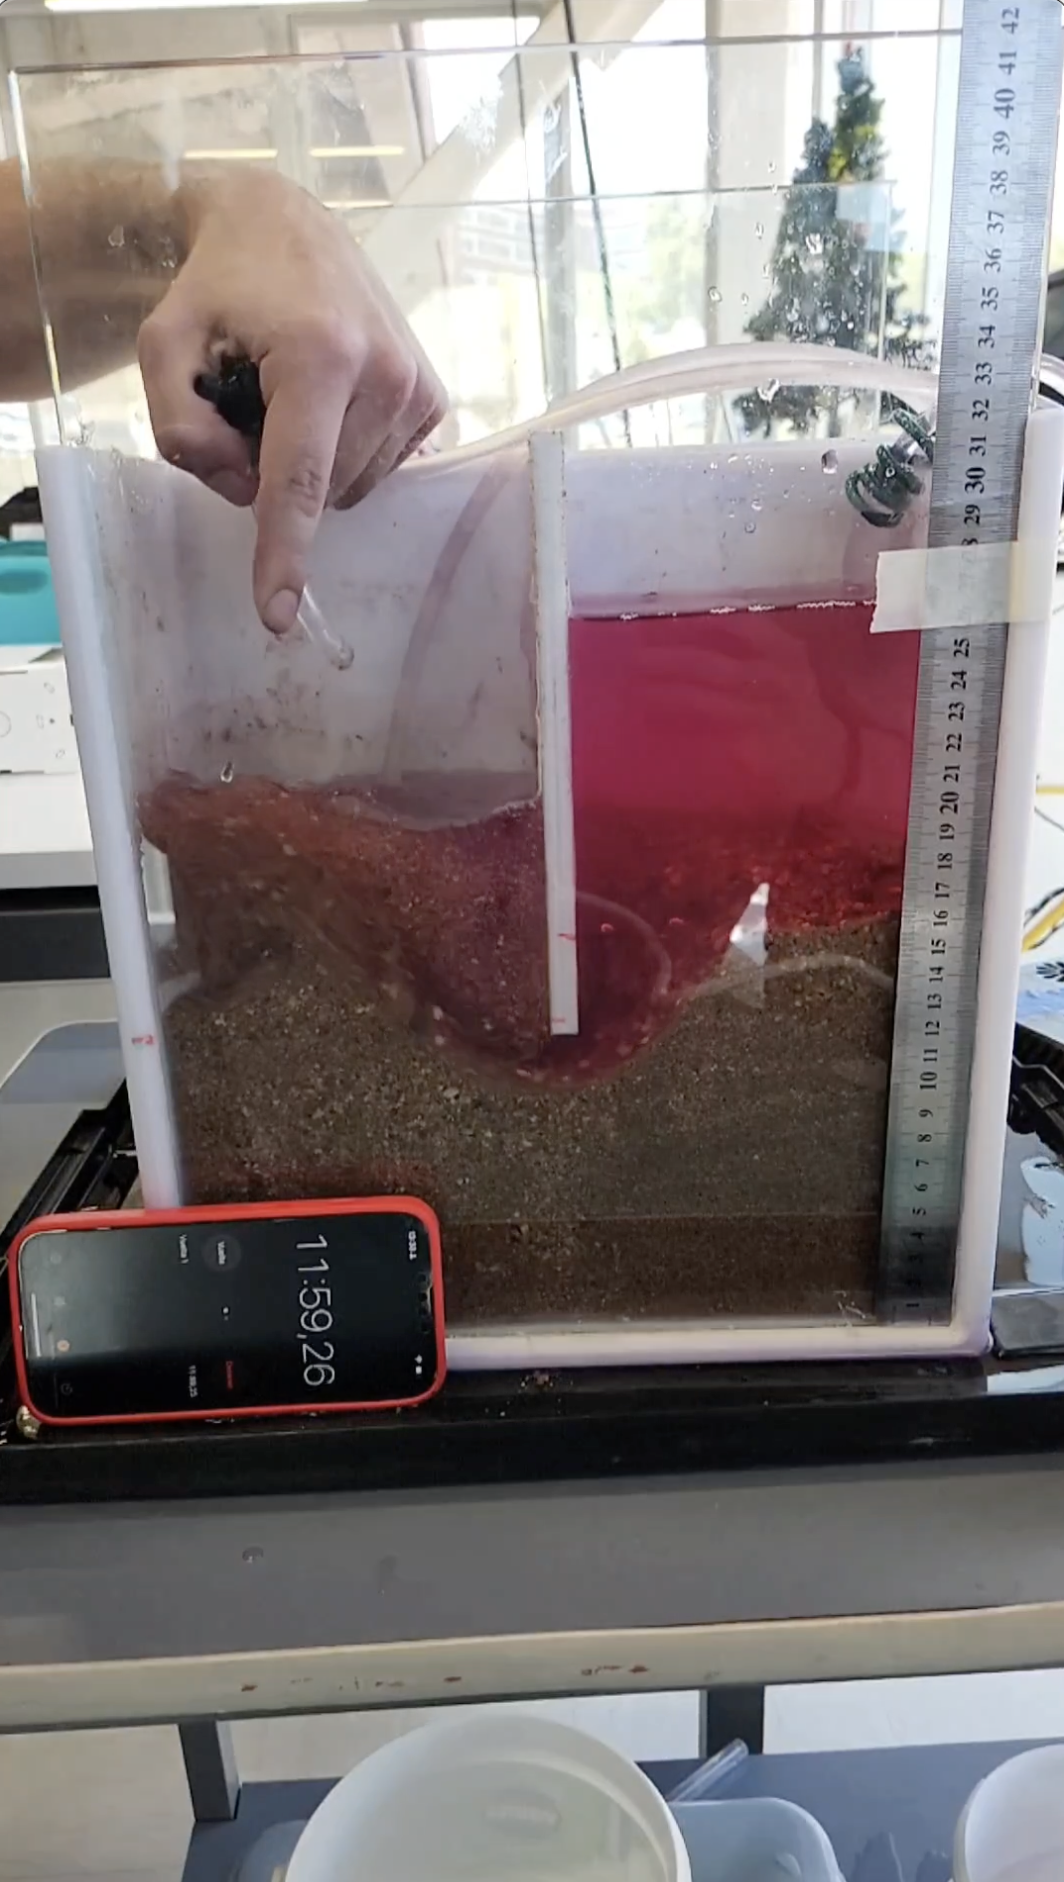
\includegraphics[width=\textwidth]{VIDEOS/miniatura_licuefaccion.png}}{VPlayer.swf}
\end{center}

Las medidas registradas son las siguientes:

\begin{table}[H]
    \centering
    \begin{tabular}{|c|c|c|c|c|c|c|c|}
    \hline
    Caso & $a_1$ & $b_1$ & $c_1$ & $a_2$ & $b_2$ & $c_2$ & $d$ \\ \hline
    Licuefacción & 0.0 & 14.5 & 15.5 & 15 & 2.5 & 12.5 & 0.5 \\ \hline
    \end{tabular}
    \caption{Medidas para la Licuefacción [cm]}
    \label{tab:medidas1}
\end{table}

Posteriormente, se realizó un mapa de calor correspondiente a la presión de poros durante la licuefacción:

\begin{figure}[H]
    \centering
    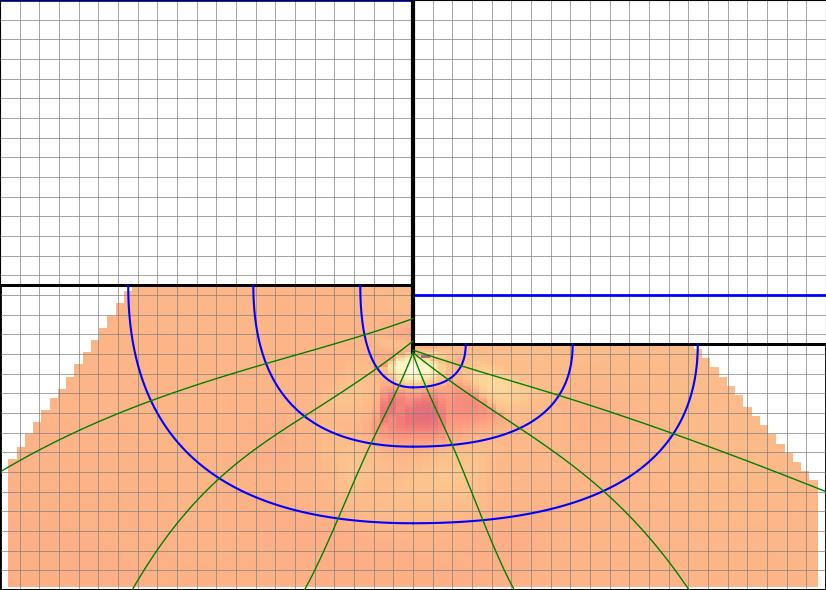
\includegraphics[width=0.5\textwidth]{GRAFICOS/caso_licuefaccion_presion_poros.jpg}
    \caption{Mapa de Calor de la Licuefacción}
    \label{fig:maqueta_licuefaccion}
\end{figure}

Es interesante notar cómo se produce un gran aumento de presión bajo la ataguía, lo cual se observa en el video, ya que ese es el punto esperado de falla.

Además, se calculó el mismo caso utilizando diferencias finitas:

\begin{figure}[H]
    \centering
    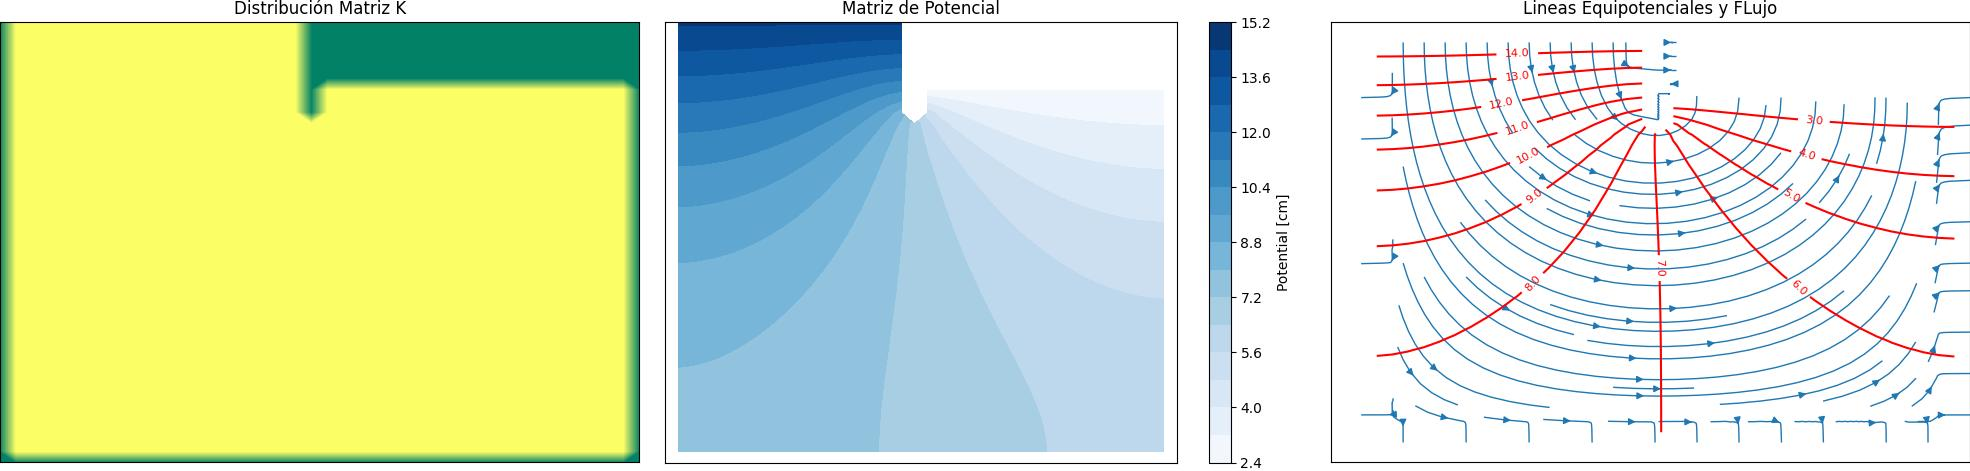
\includegraphics[width=1\textwidth]{GRAFICOS/laplace_caso_licuefaccion_escala_cm.jpg}
    \caption{Simulación con Diferencias Finitas del Caso de Licuefacción}
    \label{fig:maqueta_licuefaccion_diferencias_finitas}
\end{figure}

\subsection{Aplicación de Diferencias Finitas}

Se determinó un caudal de 0.008972885614821659 cm/s.
